%% Author: Christoph Born (53034, 22/041/62)
%% LaTeX source code of documentation

%% Author: Christoph Born (53034, 22/041/62)
%% excerpt of header-2025ss.tex

\documentclass[12pt,a4paper,twoside]{article}
\usepackage[inner=2cm,outer=3cm,top=2cm,bottom=2cm,marginpar=2.1cm]{geometry}
\usepackage[]{changepage}
\usepackage[utf8]{inputenc}
\usepackage[T1]{fontenc}
\usepackage[ngerman]{babel}
\usepackage[]{ngerman}
\usepackage[]{parskip} % "normaler" Absatzstil
\usepackage[]{enumerate}
\usepackage[]{amsmath}
\usepackage[]{amssymb}
\usepackage[]{mathtools}
\usepackage[]{graphicx}
\usepackage[bookmarks]{hyperref}
\usepackage[]{xstring}
\usepackage[]{textcomp}

% serifenlose Schrift
\renewcommand{\familydefault}{\sfdefault}

% custom \maketitle
\makeatletter
\newcommand{\module}[1]{\gdef\@module{#1}}
\newcommand{\professor}[1]{\gdef\@professor{#1}}
\newcommand{\authordetail}[1]{\gdef\@authordetail{#1}}

\author{Christoph Born}
\authordetail{}
\date{\today}

\renewcommand{\maketitle}{
	\begin{center}
		{\Large \@title\ des Moduls}\\[1.5em]
		
		{\Huge \@module}\\[1.5em]
		
		{\Large bei \@professor}\\[5em]
		
		
		{\Large \@author}
		\IfEq{\@authordetail}{}{
			\\[1em]
		}{
			\\[0.5em]
			
			\@authordetail\\[1em]
		}
		
		zuletzt geändert am \@date\\[8em]
	\end{center}
}
\makeatother

\title{Dokumentation Beleg}
\module{Programmierung 1}
\professor{Prof. Dr.-Ing. Arnold Beck}

\begin{document}

\maketitle

\tableofcontents
\newpage

\section{Aufgabenstellung}
\textbf{Matrikelnummer:} 53034 \\
\textbf{Aufgabe:} Wörterbuch deu-engl / engl-deu ($(53034 \mod 4) + 1 = 3$) \\
\textbf{Art Bedienoberfläche:} gtk+ ($(53034 \mod 3) + 1 = 1$)

\subsection{Anforderungen}
\begin{itemize}
	\item Verwaltung von Datensätzen, die Verbindung aus deutschem und englischem Wort speichern
	
	\item Operationen mit Datensätzen:
	\begin{itemize}
		\item Erfassen
		\item Löschen
		\item Suchen
		\item Anzeigen: sortierte tabellarische Auflistung aller Daten \\
		(wahlweise nach englischer/deutscher Sortierung)
	\end{itemize}
	
	\item Datenspeicherung:
	\begin{itemize}
		\item programmintern durch geeignete Datenstrukturen \\
		(Bereitstellung von Speicherbereichen in der erforderlichen Größe per malloc/free für alle verwalteten Daten, insbesondere für Zeichenketten)
		
		\item in Datei(-en) \\
		(beim Verlassen des Programms speichern, sofern sich die Daten beim Programmlauf verändert haben)
	\end{itemize}
	
	\item Programm sinnvoll in mindestens 3 C-Module eingeteilt
	\begin{itemize}
		\item getrennt kompilierbar
		\item je ein c- und Headerfile
	\end{itemize}
	
	\item Quelltexte sorgsam kommentiert (einschließlich Urheberschaft im Kopf der Quelltexte)
	
	\item Kann auf den Rechnern in den Laboren der Fakultät vorgeführt und übersetzt werden
\end{itemize}

\section{Implementierung}

\subsection{Übersicht Dateien}
\begin{itemize}
	\item beleg-prog1.glade: Layout-Definition des GTK-GUI, erstellt mit Glade \\
	Das Binärimage hängt hiervon ab, bitte stellen Sie diese Datei deshalb zur Ausführung immer im selben Ordner unter diesem Namen bereit.
	
	\item main.*, dict.*, list.*: Quelltext-Module \\
	(Beschreibung siehe jeweilige Header-Datei)
	
	\item unit\_tests/: Tests für die Module anhand vorgefertigter Szenarien \\
	(für die fertige Applikation nicht benötigt)
	\begin{itemize}		
		\item dicttest*, listtest*: Quellcode, zu erwartende Ausgabe und ggf. weitere benötigte Dateien \\
		(unit\_tests/dicttest\_assets/* können Sie als Ausgangspunkt zum Ausprobieren benutzten.)
		
		\item unit\_test.h: enthält Makros, die in den Tests genutzt werden
	\end{itemize}
\end{itemize}

\subsection{Aufbau Hauptfenster}
\begin{center}
	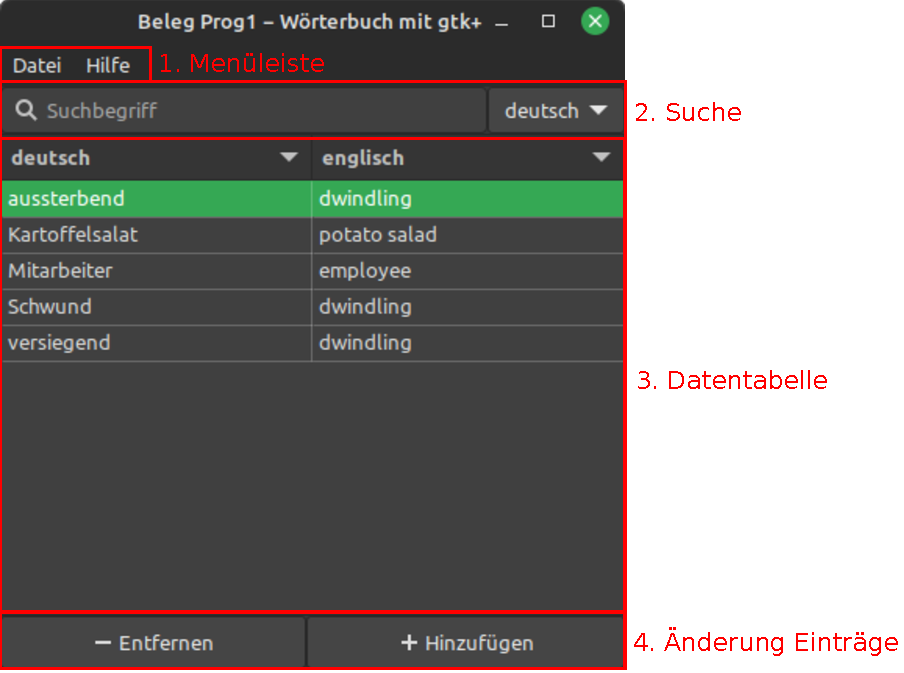
\includegraphics{Screenshot.pdf}
\end{center}
\begin{enumerate}
	\item Menüleiste: Enthält Optionen rund um das Öffnen und Speichern von Dateien, sowie Info-Dialog
	\item Suche: Bei Eingabe eines Suchbegriffs startet die Suche in den Worten der daneben gewählten Sprache
	\item Datentabelle:
	\begin{itemize}
		\item Sprache der Sortierung kann über Klick auf die Spaltenüberschrift geändert werden
		\item Reihenfolge der Spalten kann per Ziehen mit der Maus an den Überschriften geändert werden
		\item Bei Bedarf erscheint eine Scrollbar, außerdem lässt sich die Größe des Fensters mit der Maus per Ziehen an der unteren rechten Ecke ändern
	\end{itemize}
	\item Änderung Einträge:
	\begin{itemize}
		\item Bei Klick auf Entfernen wird nach Nachfrage der markierte Eintrag entfernt
		\item Bei Klick auf Hinzufügen öffnet sich ein Dialog, über den- deutsches und englisches Wort eingetragen werden können
	\end{itemize}
\end{enumerate}

\subsection{GUI-Elemente und ihre IDs in Glade}
\begin{center}
	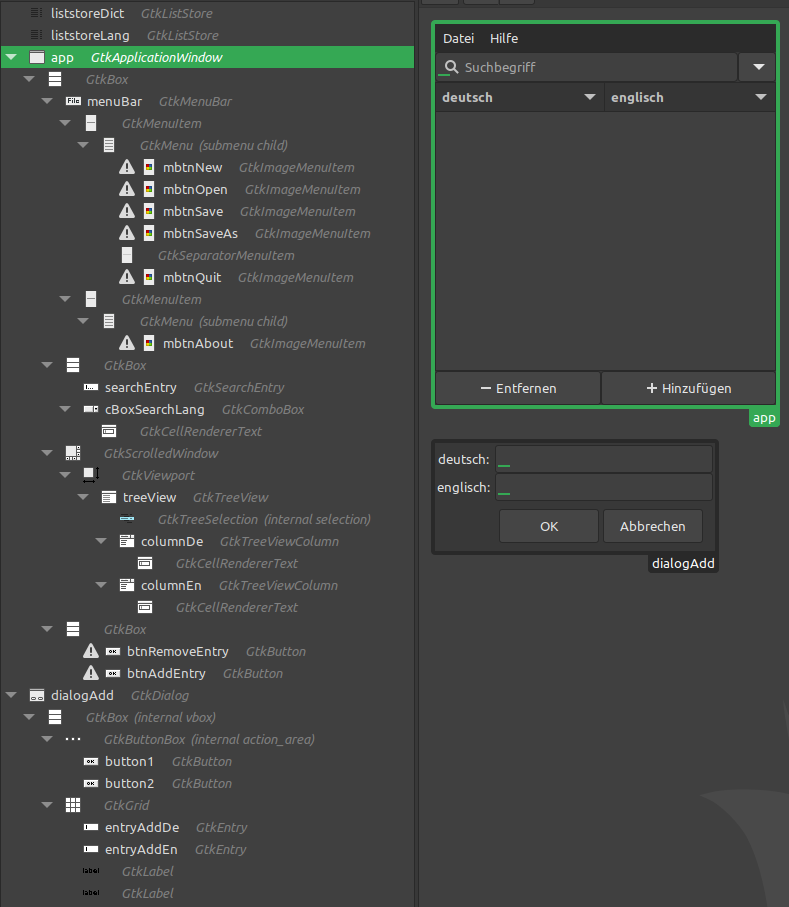
\includegraphics[width=\linewidth]{Screenshot Glade.png}
\end{center}

\end{document}